\documentclass[a4paper,11pt]{article}
\usepackage[margin=1.0in]{geometry}
\usepackage{graphicx}
\usepackage{subcaption}
\usepackage{amsmath}
\usepackage{float}
\usepackage{indentfirst}
\usepackage{array}
\newcolumntype{P}[1]{>{\centering\arraybackslash}p{#1}}

\begin{document}
\title{Economics 582: Replication Study - Krueger (1999)}
\author{Marissa Reuther}
\date{December 2nd, 2019}
\maketitle

\subsection*{I. Introduction}
This paper replicates various results from Alan Krueger's paper\footnote{Krueger, A. (1999). Experimental Estimates of Education Production Functions. \textit{The Quarterly Journal of Economics}, 114(2), 497-532. Retrieved from www.jstor.org/stable/2587015}  studying the effects of class size on student achievement. In order to do this, Krueger studies the effects of the Tennessee Student/Teacher Achievement Ratio Experiment (Project STAR). This policy started in 1985 and randomly assigned students and teachers across 80 schools to small and regular class sizes. \par

The outcome of interest Krueger’s study is student achievement level, which is specifically measured through student scores on two standardized tests (the SAT and the Tennessee Basic Skills First (BSF)). Studying the effects of these standardized test scores are important because they are a significant part of what dictates students’ future educational attainment, such as getting into better colleges and universities.  \par

Krueger studies several factors that could potentially affect student achievement. In this paper, class size is the main independent variable of interest. He hypothesizes, based on previous work pertaining to Project STAR, that students assigned to smaller classes tend to have better standardized test scores, holding all else constant. Various specifications throughout the paper support this hypothesis. \par

Krueger also analyzes the effects of some other independent variables such as teacher ability and whether a classroom had a full-time teacher aid present. These results do not appear to have much impact on test scores. \par

To measure standardized test scores, Krueger creates an average percentile score based on the reading, math, and word skills tests. For his main analysis, he uses percentiles based only on SAT scores. Later in the paper, he alters the model by using percentiles only from BSF scores and did not find much difference in the results. In both the SAT and BSF scores, a higher percentile corresponds to a student with a higher achievement level. \par

For class size in the main analysis, Krueger uses a categorical variable to describe the class size the student was randomly placed into each year. The three categories were small (13-17 students), regular (22-25 students) and regular/aid (22-25 students and a teacher aid).  \par

If Project STAR had not used randomization for assigning students to class types, Krueger would have needed a conditional independence assumption to be able to interpret the effects of class size on student achievement as causal. For conditional independence, unobserved characteristics within the error term need to be uncorrelated with the regressors of interest, after holding all other characteristics constant. In the context of this paper, there cannot be any unobservable characteristics correlated with class size. \par

In the case of a non-randomized experiment, omitted variables could violate the conditional independence assumption, such as student’s inherent ability. Students who are ‘over-achievers’ or who may be smarter than others will have inherent ability correlated with standardized test scores. Additionally, their inherent ability can be correlated with class size if they are placed in ‘gifted’ programs or are given some similar small class size advantage over those with lower inherent ability. \par

For this experiment, Project STAR used randomization for placing students in different class types to overcome possible omitted variable bias. If class size was truly determined randomly, then it should also be randomizing the distribution of student’s inherent abilities. This randomization should make class size uncorrelated with inherent ability and other unobservable characteristics, thus eliminating any potential omitted variable bias and allowing results to be interpreted as causal. \\

\subsection*{II. Data}
The data used in this paper and replication can be found on the Harvard Dataverse\footnote{C.M. Achilles; Helen Pate Bain; Fred Bellott; Jayne Boyd-Zaharias; Jeremy Finn; John Folger; John Johnston; Elizabeth Word, 2008, "Tennessee's Student Teacher Achievement Ratio (STAR) project"} \par
The data consists of 11,600 observations, each corresponding to a student in Project STAR. The study focused on the same set of 80 schools  starting in 1985, and followed the students in those schools from kindergarten through high school. \par
The study tracked class types the students were randomly assigned to, as well as several other observable characteristics such as race, gender, birthday, free lunch status, standardized test scores, and actual class size.\par

The study also tracked teacher characteristics such as race, gender, years of experience, and highest degree achieved. \\

\subsection*{III. Results 1}

\subsubsection*{III.i Table 1}
The replication of Table 1 from Krueger's paper are summarized by Table 1.A and Table 1.B below. These results are used to check how well Project STAR randomized students into the three class types. Because the students were randomly assigned to class types, we would expect the means of the controls to be equal across class types. If the results suggest that randomization was not perfect, it would threaten our ability to interpret the results as causal.
 \par

Table 1.A reports the mean characteristics across controls, actual class size, and the outcome variable. Each grade panel corresponds to when the student first entered the Project STAR. For example, among students who entered STAR in Kindergarten, 47.1\% of the students in small classes qualified for free lunch. \par

Table 1.B reports the p-value for the joint hypothesis test that the means across class types for each variable are equal. For control variables, we would expect the means across class types to be equal. For class size and percentiles, we would expect the means across class types to be different. Because of this, if Project STAR were perfectly randomized and class size was correlated with test scores, we would expect to fail to reject ($p >$ 0.01 at the 1\% significance level) all the null hypothesis for controls, and reject ($p <$ 0.01) all the hull hypothesis for class size and percentiles. While this is true for some of the results, it does not hold for every variable across the grades. Because of this, Krueger adjusts the data and reports those results in Table 2. \par



\begin{table}[H]
\begin{center}
\begin{tabular}{l|llllll} 
	\multicolumn{7}{c}{Table 1.A: Mean Characteristics of Treatments and Controls: Unadjusted Data} \\ \hline \hline
	\textbf{Kindergarten} & Free Lunch  & White/Asian  & Age in 1985  & Attrition  & Class-Size  & Percentile  \\  \hline 
	Small & 0.471 & 0.683 & 5.442 & 0.487 & 15.117 & 54.730 \\  
	Regular & 0.477 & 0.675 & 5.426 & 0.518 & 22.383 & 49.955 \\  
	Regular/Aide & 0.503 & 0.659 & 5.432 & 0.529 & 22.774 & 49.984 \\ \hline \hline
	\textbf{1st Grade}& Free Lunch  & White/Asian  & Age in 1985  & Attrition  & Class-Size  & Percentile  \\  \hline 
	Small & 0.592 & 0.622 & 5.778 & 0.527 & 15.87 & 49.462 \\  
	Regular & 0.624 & 0.562 & 5.858 & 0.513 & 22.71 & 42.896 \\  
	Regular/Aide & 0.607 & 0.651 & 5.876 & 0.468 & 23.457 & 48.033 \\ \hline \hline   
	\textbf{2nd Grade} & Free Lunch  & White/Asian  & Age in 1985  & Attrition  & Class-Size  & Percentile  \\  \hline 
	Small & 0.655 & 0.574 & 5.881 & 0.369 & 15.500 & 46.593 \\  
	Regular & 0.633 & 0.567 & 5.908 & 0.336 & 23.714 & 45.419 \\  
	Regular/Aide & 0.659 & 0.465 & 5.939 & 0.349 & 23.592 & 41.813 \\  \hline \hline 
	\textbf{3rd Grade} & Free Lunch  & White/Asian  & Age in 1985  & Attrition  & Class-Size  & Percentile  \\  \hline 
	Small & 0.598 & 0.668 & 5.952 & NA & 15.971 & 47.873 \\  
	Regular & 0.645 & 0.577 & 5.929 & NA & 24.051 & 44.522 \\  
	Regular/Aide & 0.686 & 0.558 & 5.986 & NA & 24.425 & 41.558 \\  
	\hline \hline 
\end{tabular}
\end{center}
\end{table}

\begin{table}[H]
\begin{center}	
	\begin{tabular}{ l | l  l  l  l } 
	\multicolumn{5}{c}{Table 1.B: P Values of Mean Equality for} \\
	\multicolumn{5}{c}{Treatments and Controls: Unadjusted Data} \\ \hline \hline
	& K  & 1  & 2  & 3  \\  \hline 
	Free Lunch & 0.088 & 0.518 & 0.605 & 0.038 \\  
	White/Asian & 0.251 & 0.000 & 0.000 & 0.003 \\  
	Age in 1985 & 0.335 & 0.033 & 0.405 & 0.498 \\  
	Attrition & 0.024 & 0.069 & 0.580 & NA \\  
	Class-Size & 0.000 & 0.000 & 0.000 & 0.000 \\  
	Percentile & 0.000 & 0.000 & 0.010 & 0.006 \\  
\hline \hline
\end{tabular}
\end{center}
\end{table}


\subsubsection*{III.ii Table 2}
Table 2 reports the results for the same hypothesis test as Table 1, but also controls for school effects. This allows for heterogeneity across schools. \par
These results are more consistent with the relationship we would expect to see, and as was described in the section above. We can reject the hypothesis that the means across class types are equal for every control except attrition in first grade. There are also significant differences in class sizes and percentile scores, except for 2nd grade percentiles.  \par
This table provides evidence for supporting controlling school effects in the rest of the paper's analysis. \par

\begin{table}[H]
\begin{center}	
\centering
	\begin{tabular}{ l | l  l  l  l } 
	\multicolumn{5}{c}{Table 2: P Values for Within School} \\
	\multicolumn{5}{c}{Differences Among Class Types} \\ \hline \hline
	& K  & 1  & 2  & 3  \\  \hline 
	Free Lunch & 0.446 & 0.292 & 0.579 & 0.184 \\  
	White/Asian & 0.647 & 0.276 & 0.710 & 0.369 \\  
	Age in 1985 & 0.438 & 0.120 & 0.435 & 0.477 \\  
	Attrition & 0.012 & 0.370 & 0.848 & NA \\  
	Class-Size & 0.000 & 0.000 & 0.000 & 0.000 \\  
	Percentile & 0.000 & 0.000 & 0.429 & 0.004 \\  
	\hline \hline
\end{tabular}
\end{center}
\end{table}


\subsubsection*{III.iii Table 3}	
Table 3 shows the distribution of children across actual class sizes by random assignment group in first grade. This shows that even through the class types typically fall into the intended class ranges from Project STAR, there is a large range within each class type. Because of this, Krueger later runs a two stage least squares regression using actual class size as an instrument for class type. 

\begin{table}[H]
\centering
\begin{tabular}{P{2cm}|P{2cm}P{2cm}P{2cm}}
	\multicolumn{4}{c}{Table 3: Distribution of Children Across Actual Class }\\
	\multicolumn{4}{c}{Sizes by Random Assignment Group in First Grade} \\  \hline \hline
	Actual Class-Size& Small  & Regular  & Regular/Aide  \\  \hline 
	12 & 24 & 0 & 0 \\  
	13 & 182 & 0 & 0 \\  
	14 & 252 & 0 & 0 \\  
	15 & 465 & 0 & 0 \\  
	16 & 256 & 16 & 0 \\  
	17 & 561 & 17 & 0 \\  
	18 & 108 & 36 & 0 \\  
	19 & 57 & 76 & 57 \\  
	20 & 20 & 200 & 120 \\  
	21 & 0 & 378 & 378 \\  
	22 & 0 & 594 & 330 \\  
	23 & 0 & 437 & 460 \\  
	24 & 0 & 384 & 264 \\  
	25 & 0 & 175 & 225 \\  
	26 & 0 & 130 & 234 \\  
	27 & 0 & 54 & 108 \\  
	28 & 0 & 28 & 56 \\  
	29 & 0 & 29 & 58 \\  
	30 & 0 & 30 & 30 \\  \hline \hline
	Average &  15.697 & 22.697 & 23.436 \\  
	\hline \hline 
\end{tabular}
\end{table}
	

\subsubsection*{III.iv Figure 1}
Figure 1 shows the distribution of average SAT scores in small classes and regular classes across the four grades. \par
Each density plot shows the expected relationship that supports Krueger's hypothesis. Small classes had more students scoring in higher percentiles, and regular classes had more students scoring in lower percentiles.  
	
\begin{figure}[H]
\begin{subfigure}{0.5\textwidth}
	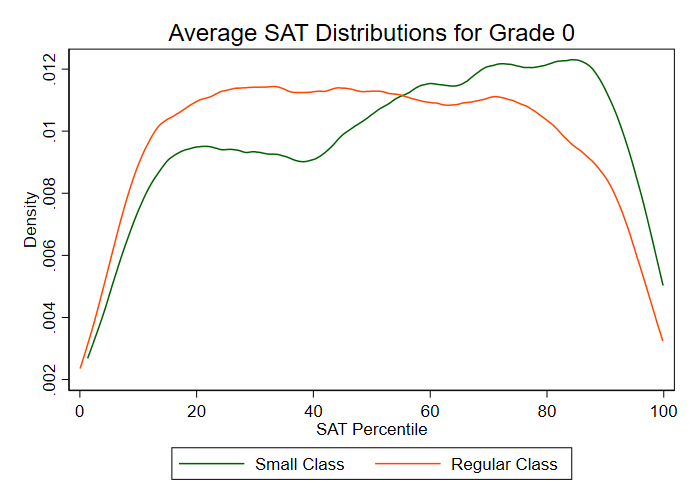
\includegraphics[width=\linewidth]{figure1_0.png}
\end{subfigure}
\begin{subfigure}{0.5\textwidth}
	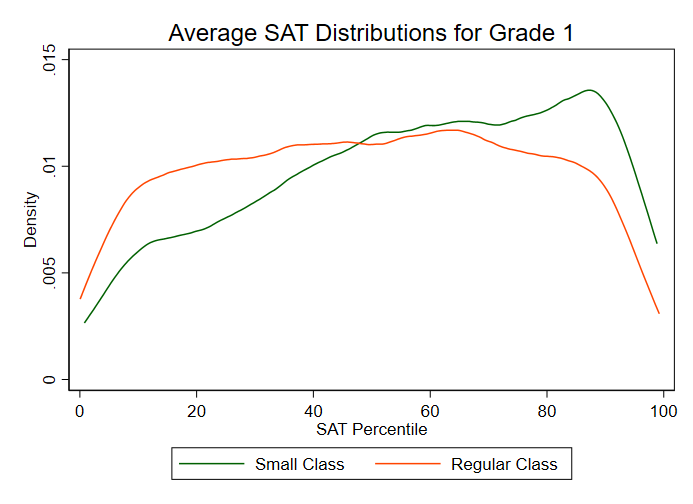
\includegraphics[width=\linewidth]{figure1_1.png}
\end{subfigure}
\end{figure}
\begin{figure}[H]
\begin{subfigure}{0.5\textwidth}
	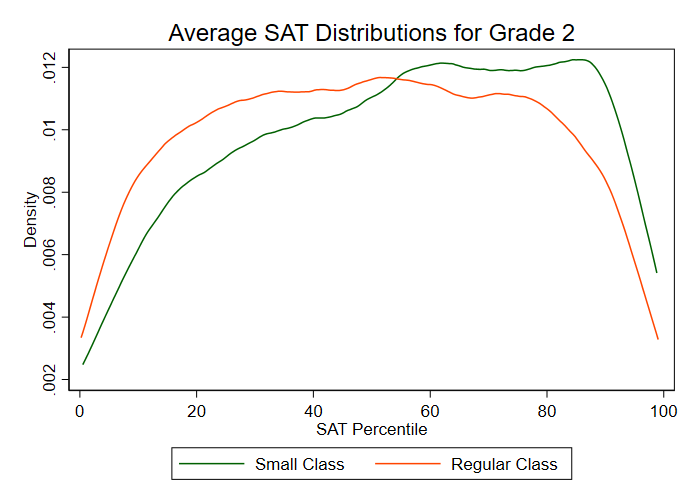
\includegraphics[width=\linewidth]{figure1_2.png}
\end{subfigure}
\begin{subfigure}{0.5\textwidth}
	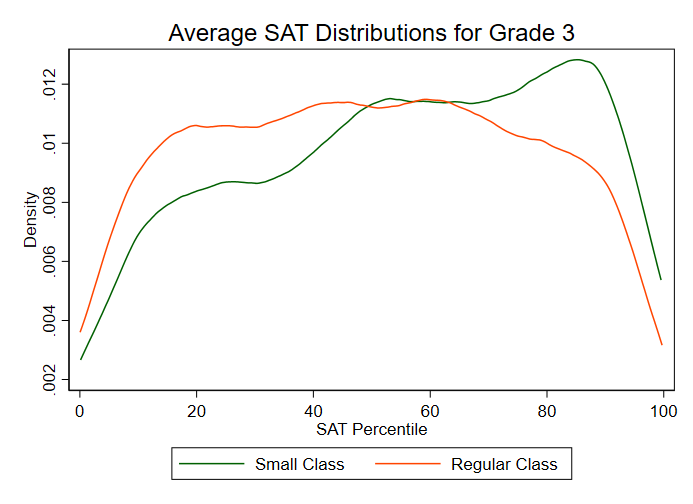
\includegraphics[width=\linewidth]{figure1_3.png}
\end{subfigure}
\end{figure} 



\subsection*{IV. Empirical Design}
This paper replicates the results of Table 5 and Table 7. All of these results can be interpreted as causal as long as Project STAR made assignments that were truly random. \par

Table 5 estimates the following equation: 
\begin{align}
 Y_{ics} = \beta_{0} + \beta_{1}SMALL_{cs} + \beta_{2}REG/A_{cs} + \beta_{3}X{ics} + \alpha_{s} + \epsilon_{ics}
\end{align}

$Y_{ics}$ is the average percentile score of student $i$ in classroom $c$ at school $s$. $SMALL_{cs}$ is an indicator for a student assigned to a small size classroom, and $REG/A_{cs}$ is an indicator for a student assigned to a regular class type with a teacher aide.  $\beta_{1}$ will capture the mean difference in percentile scores for students in small classes compared to students in regular classes. $\beta_{2}$ will capture the mean difference in percentile scores for students in regular classes with an aide compared to students in regular classes with no aide. $X_{ics}$ is a vector of controls for observable student and teacher characteristics. Randomization should already control for these differences, so we would expect $\beta_{3}$ estimates to be relatively small. $\alpha_{s}$ is a vector of school indicators to account for school fixed effects. \par

Table 5 uses two OLS models to estimate equation (1). Both models have 4 different specifications. The first specification has no control variables. The second specification controls for school effects. The third specification controls for school effects and observable student differences. The fourth specification controls for school effects and observable student and teacher differences. In every specification, standard errors are clustered by classroom level. Regressions are created for each of the four grades, kindergarten through third. \par

The first model of Table 5 regresses percentile scores on indicator variables for small class type and regular/aide class type.  The second model of Table 5 is a reduced form model. This model uses initial class assignment rather than actual class assignment to see if student's switching class types altered the results from the initial randomization. \par

Table 7 estimates the following system:
\begin{align}
CS_{ics} = \pi_{0} + \pi_{1}S_{ios} + \pi_{2}R_{ios} + \pi_{3}X_{ics} + \delta_{s} + \tau_{ics}
\end{align}
\begin{align}
Y_{ics} = \beta_{0} + \beta_{1}CS_{ics} + \beta_{2}X_{ics} + \alpha_{s} + \epsilon_{ics}
\end{align}

$CS_{ics}$ is actual class size the student was in each year. $S_{ios}$ is an initial assignment to a small class. $R_{ios}$ is an initial assignment to a regular class.  \par

First, Krueger uses an OLS regression to estimate equation (2) and then he uses 2SLS to model equations (2) and (3), with initial class type assignments as an instrument for class size. In both cases, he control for school effects and teacher and student observable differences. \par 

As shown by Table 3, there is a large distribution of actual class sizes within the three class types. Because of this, results of Table 7 should more accurately capture the effects of class size on test scores. \par
The OLS model directly inputs class size in the regression. The 2SLS model uses initial class type assignments as an instrument for class size to account for possible endogeneity of class size on percentile scores. For example, some parents may push for their students to get placed into smaller class sizes as Project STAR progressed. Because of this, class size may not always be purely random and may become endogenous as time goes on. Using 2SLS to instrument class size based in initial class type assignments will limit these effects and ensure we can interpret estimates as causal. Moreover, OLS and 2SLS estimates will likely be slightly different. \\ \\  	

\subsection*{V. Results 2}

\subsubsection*{V.i Table 5}
The results of Table 5 are summarized below. A separate table was created for each grade. In each grade, small class had a positive statistically significant effect on average SAT percentile scores.\par

\begin{table}[H]
	\setlength\tabcolsep{1.75pt} 
\begin{tabular*}{\textwidth}{@{\extracolsep{\fill}}lcccccccc}				
	& \multicolumn{4}{c}{OLS}  & \multicolumn{4}{c}{Reduced Form}\\
	\cline{2-5}	\cline{6-9}			
	Table 5: Kindergarten & \multicolumn{1}{c}{(1)\mbox{\ }} &	\multicolumn{1}{c}{(2)\mbox{\ }} &	\multicolumn{1}{c}{(3)\mbox{\ }} &	\multicolumn{1}{c}{(4)} & \multicolumn{1}{c}{(5)\mbox{\ }} &	\multicolumn{1}{c}{(6)\mbox{\ }} &	\multicolumn{1}{c}{(7)\mbox{\ }} &	\multicolumn{1}{c}{(8)} \\
	\hline				
	Small Class &	4.778 &	5.341 &	5.392 &	5.327  & 4.778 &	5.341 &	5.392 &	5.327\\
	&	\raisebox{.7ex}[0pt]{\scriptsize (2.190)$^{**}$} &	\raisebox{.7ex}[0pt]{\scriptsize (1.266)$^{***}$} &	\raisebox{.7ex}[0pt]{\scriptsize (1.221)$^{***}$} &	\raisebox{.7ex}[0pt]{\scriptsize (1.200)$^{***}$} &	\raisebox{.7ex}[0pt]{\scriptsize (2.190)$^{**}$} &	\raisebox{.7ex}[0pt]{\scriptsize (1.266)$^{***}$} &	\raisebox{.7ex}[0pt]{\scriptsize (1.221)$^{***}$} &	\raisebox{.7ex}[0pt]{\scriptsize (1.200)$^{***}$} \\
	Regular + Aide Class &	0.064 &	0.215 &	0.457 &	0.258 &	0.064 &	0.215 &	0.457 &	0.258 \\
	&	\raisebox{.7ex}[0pt]{\scriptsize (2.219)} &	\raisebox{.7ex}[0pt]{\scriptsize (1.126)} &	\raisebox{.7ex}[0pt]{\scriptsize (1.096)} &	\raisebox{.7ex}[0pt]{\scriptsize (1.068)} 	&	\raisebox{.7ex}[0pt]{\scriptsize (2.219)} &	\raisebox{.7ex}[0pt]{\scriptsize (1.126)} &	\raisebox{.7ex}[0pt]{\scriptsize (1.096)} &	\raisebox{.7ex}[0pt]{\scriptsize (1.068)}\\
	White/Asian &	&	&	8.316 &	8.372 &	&	&	8.316 &	8.372  \\
	&	&	&	\raisebox{.7ex}[0pt]{\scriptsize (1.353)$^{***}$} &	\raisebox{.7ex}[0pt]{\scriptsize (1.362)$^{***}$} 	&	&	&	\raisebox{.7ex}[0pt]{\scriptsize (1.353)$^{***}$} &	\raisebox{.7ex}[0pt]{\scriptsize (1.362)$^{***}$}\\
	Girl &	&	&	4.399 &	4.371 &	&	&	4.399 &	4.371 \\
	&	&	&	\raisebox{.7ex}[0pt]{\scriptsize (0.631)$^{***}$} &	\raisebox{.7ex}[0pt]{\scriptsize (0.632)$^{***}$} &	&	&	\raisebox{.7ex}[0pt]{\scriptsize (0.631)$^{***}$} &	\raisebox{.7ex}[0pt]{\scriptsize (0.632)$^{***}$}\\
	Free Lunch &	&	&	-13.128 &	-13.078  &	&	&	-13.128 &	-13.078\\
	&	&	&	\raisebox{.7ex}[0pt]{\scriptsize (0.771)$^{***}$} &	\raisebox{.7ex}[0pt]{\scriptsize (0.775)$^{***}$} &	&	&	\raisebox{.7ex}[0pt]{\scriptsize (0.771)$^{***}$} &	\raisebox{.7ex}[0pt]{\scriptsize (0.775)$^{***}$}\\
	White Teacher &	&	&	&	-1.137  &	&	&	&	-1.137\\
	&	&	&	&	\raisebox{.7ex}[0pt]{\scriptsize (2.169)} 	&	&	&	&	\raisebox{.7ex}[0pt]{\scriptsize (2.169)} \\
	Male Teacher &	&	&	&	 &	&	&	&	\\
	&	&	&	& &	&	&	&		\\
	Teacher Experience &	&	&	&	0.263  &	&	&	&	0.263 \\
	&	&	&	&	\raisebox{.7ex}[0pt]{\scriptsize (0.106)$^{**}$} 	&	&	&	&	\raisebox{.7ex}[0pt]{\scriptsize (0.106)$^{**}$}\\
	Master's Degree &	&	&	&	-.578 &	&	&	&	-.578\\
	&	&	&	&	\raisebox{.7ex}[0pt]{\scriptsize (1.062)}&	&	&	&	\raisebox{.7ex}[0pt]{\scriptsize (1.062)} \\
	School Fixed Effects &	No  & Yes &	Yes & Yes &	No & Yes &	Yes & Yes \\
	R\textsuperscript{2} & 0.007 & 0.244 & 0.305 & 0.309 & 0.032 & 0.244 & 0.305 & 0.309\\
	Obs. &	5901 &	5901 &	5882 &	5839  &	5901 &	5901 &	5882 &	5839 \\
	\hline\hline				
\end{tabular*}		
\end{table}		

In Kindergarten, OLS and reduced form estimates are equal because initial assignments are the same as actual assignments. Students in small classes had higher scores on average by 5.327 percentile points compared to students in regular classes. The effect of a teacher's aide is not significant, suggesting that there was no difference in test scores for students in regular classes and regular classes with an aide. White and Asian students had higher average test scores by 8.37 percentile points. Female students had higher average test scores by 4.371 percentile points. Students who qualified for free lunch had lower average test scores by 13.079 percentile  points. These three student control effects are significant at the 1 percent level. Teacher experience has a small positive effect on test scores by 0.263 percentile points. \par

\begin{table}[H]
	\setlength\tabcolsep{1.75pt} 
\begin{tabular*}{\textwidth}{@{\extracolsep{\fill}}lcccccccc}			& \multicolumn{4}{c}{OLS}  & \multicolumn{4}{c}{Reduced Form}\\
	\cline{2-5}	\cline{6-9}			
	Table 5: 1st Grade & \multicolumn{1}{c}{(1)\mbox{\ }} &	\multicolumn{1}{c}{(2)\mbox{\ }} &	\multicolumn{1}{c}{(3)\mbox{\ }} &	\multicolumn{1}{c}{(4)} & \multicolumn{1}{c}{(5)\mbox{\ }} &	\multicolumn{1}{c}{(6)\mbox{\ }} &	\multicolumn{1}{c}{(7)\mbox{\ }} &	\multicolumn{1}{c}{(8)} \\
	\hline								
	Small Class &	8.816 &	8.513 &	7.880 &	7.355 &	7.631 &	7.086 &	6.728 &	6.321  \\
	&	\raisebox{.7ex}[0pt]{\scriptsize (1.952)$^{***}$} &	\raisebox{.7ex}[0pt]{\scriptsize (1.186)$^{***}$} &	\raisebox{.7ex}[0pt]{\scriptsize (1.165)$^{***}$} &	\raisebox{.7ex}[0pt]{\scriptsize (1.181)$^{***}$}	&	\raisebox{.7ex}[0pt]{\scriptsize (1.751)$^{***}$} &	\raisebox{.7ex}[0pt]{\scriptsize (1.124)$^{***}$} &	\raisebox{.7ex}[0pt]{\scriptsize (1.100)$^{***}$} &	\raisebox{.7ex}[0pt]{\scriptsize (1.108)$^{***}$} \\
	Regular + Aide Class &	3.483 &	2.236 &	2.190 &	1.736 &	1.910 &	1.607 &	1.631 &	1.483\\
	&	\raisebox{.7ex}[0pt]{\scriptsize (2.032)$^{*}$} &	\raisebox{.7ex}[0pt]{\scriptsize (0.976)$^{**}$} &	\raisebox{.7ex}[0pt]{\scriptsize (0.975)$^{**}$} &	\raisebox{.7ex}[0pt]{\scriptsize (0.972)$^{*}$} &	\raisebox{.7ex}[0pt]{\scriptsize (1.104)$^{*}$} &	\raisebox{.7ex}[0pt]{\scriptsize (0.795)$^{**}$} &	\raisebox{.7ex}[0pt]{\scriptsize (0.753)$^{**}$} &	\raisebox{.7ex}[0pt]{\scriptsize (0.756)$^{**}$}  \\
	White/Asian &	&	&	6.932 &	6.923&	&	&	6.815 &	6.801 \\
	&	&	&	\raisebox{.7ex}[0pt]{\scriptsize (1.188)$^{***}$} &	\raisebox{.7ex}[0pt]{\scriptsize (1.195)$^{***}$} 	&	&	&	\raisebox{.7ex}[0pt]{\scriptsize (1.187)$^{***}$} &	\raisebox{.7ex}[0pt]{\scriptsize (1.194)$^{***}$} \\
	Girl &	&	&	3.809 &	3.844  &	&	&	3.774 &	3.815\\
	&	&	&	\raisebox{.7ex}[0pt]{\scriptsize (0.563)$^{***}$} &	\raisebox{.7ex}[0pt]{\scriptsize (0.563)$^{***}$} &	&	&	\raisebox{.7ex}[0pt]{\scriptsize (0.561)$^{***}$} &	\raisebox{.7ex}[0pt]{\scriptsize (0.561)$^{***}$} \\
	Free Lunch &	&	&	-13.465 &	-13.604  &	&	&	-13.626 &	-13.768  \\
	&	&	&	\raisebox{.7ex}[0pt]{\scriptsize (0.872)$^{***}$} &	\raisebox{.7ex}[0pt]{\scriptsize (0.872)$^{***}$} 	&	&	&	\raisebox{.7ex}[0pt]{\scriptsize (0.874)$^{***}$} &	\raisebox{.7ex}[0pt]{\scriptsize (0.872)$^{***}$}\\
	White Teacher &	&	&	&	-4.289 &	&	&	&	-4.405\\
	&	&	&	&	\raisebox{.7ex}[0pt]{\scriptsize (1.959)$^{**}$} 	&	&	&	&	\raisebox{.7ex}[0pt]{\scriptsize (1.969)$^{**}$}\\
	Male Teacher &	&	&	&	11.516&	&	&	&	12.771  \\
	&	&	&	&	\raisebox{.7ex}[0pt]{\scriptsize (3.299)$^{***}$} 	&	&	&	&	\raisebox{.7ex}[0pt]{\scriptsize (3.345)$^{***}$}\\
	Teacher Experience &	&	&	&	0.054 &	&	&	&	0.063\\
	&	&	&	&	\raisebox{.7ex}[0pt]{\scriptsize (0.06)}&	&	&	&	\raisebox{.7ex}[0pt]{\scriptsize (0.06)} \\
	Master's Degree &	&	&	&	0.461&	&	&	&	0.609 \\
	&	&	&	&	\raisebox{.7ex}[0pt]{\scriptsize (1.067)} &	&	&	&	\raisebox{.7ex}[0pt]{\scriptsize (1.088)}\\
	School Fixed Effects &	No  & Yes &	Yes & Yes &	No & Yes &	Yes & Yes \\
	R\textsuperscript{2} & 0.1018 & 0.235 & 0.297 & 0.300 & 0.013 & 0.230 & 0.293 & 0.297 \\
	Obs. &	6635 &	6635 &	6465 &	6452  &	6635 &	6635 &	6465 &	6452\\
	\hline\hline				
\end{tabular*}
\end{table}
In first grade, OLS estimates are larger than the reduced form estimates. This is because OLS estimates allow for students to switch from their initial assignment. Smarter students may have switched form a regular class to a smaller class due to teacher or parental interference. This would lead OLS estimates to be larger, so reduced form estimates will eliminate this effect. The effect of class size is slightly larger in magnitude than in Kindergarten. Students in classes with an aide had higher average percentile scores by 1.483 percentile points compared to students in a regular class without an aide. The student control variables show the same relationship as in Kindergarten. Students with a white teacher had lower test scores by 4.405 percentile points. Students with a male teacher had higher average test scores by 12.771 points. \par

\begin{table}[H]
	\setlength\tabcolsep{1.75pt} 
\begin{tabular*}{\textwidth}{@{\extracolsep{\fill}}lcccccccc}		
	& \multicolumn{4}{c}{OLS}  & \multicolumn{4}{c}{Reduced Form}\\
	\cline{2-5}	\cline{6-9}			
	Table 5: 2nd Grade & \multicolumn{1}{c}{(1)\mbox{\ }} &	\multicolumn{1}{c}{(2)\mbox{\ }} &	\multicolumn{1}{c}{(3)\mbox{\ }} &	\multicolumn{1}{c}{(4)} & \multicolumn{1}{c}{(5)\mbox{\ }} &	\multicolumn{1}{c}{(6)\mbox{\ }} &	\multicolumn{1}{c}{(7)\mbox{\ }} &	\multicolumn{1}{c}{(8)} \\
	\hline			
	Small Class &	5.643 &	6.136 &	5.690 &	5.735 &	5.332 &	5.615 &	5.269 &	5.243 \\
	&	\raisebox{.7ex}[0pt]{\scriptsize (1.940)$^{***}$} &	\raisebox{.7ex}[0pt]{\scriptsize (1.258)$^{***}$} &	\raisebox{.7ex}[0pt]{\scriptsize (1.219)$^{***}$} &	\raisebox{.7ex}[0pt]{\scriptsize (1.230)$^{***}$} 	&	\raisebox{.7ex}[0pt]{\scriptsize (1.654)$^{***}$} &	\raisebox{.7ex}[0pt]{\scriptsize (1.119)$^{***}$} &	\raisebox{.7ex}[0pt]{\scriptsize (1.091)$^{***}$} &	\raisebox{.7ex}[0pt]{\scriptsize (1.097)$^{***}$} \\
	Regular + Aide Class &	1.028 &	1.338 &	1.349 &	1.480  &	-.109 &	1.062 &	1.077 &	1.157 \\
	&	\raisebox{.7ex}[0pt]{\scriptsize (2.029)} &	\raisebox{.7ex}[0pt]{\scriptsize (1.113)} &	\raisebox{.7ex}[0pt]{\scriptsize (1.077)} &	\raisebox{.7ex}[0pt]{\scriptsize (1.063)} 	&	\raisebox{.7ex}[0pt]{\scriptsize (1.204)} &	\raisebox{.7ex}[0pt]{\scriptsize (0.852)} &	\raisebox{.7ex}[0pt]{\scriptsize (0.804)} &	\raisebox{.7ex}[0pt]{\scriptsize (0.803)} \\
	White/Asian &	&	&	6.448 &	6.480&	&	&	6.363 &	6.401 \\
	&	&	&	\raisebox{.7ex}[0pt]{\scriptsize (1.192)$^{***}$} &	\raisebox{.7ex}[0pt]{\scriptsize (1.189)$^{***}$} 
	&	&	&	\raisebox{.7ex}[0pt]{\scriptsize (1.200)$^{***}$} &	\raisebox{.7ex}[0pt]{\scriptsize (1.197)$^{***}$}\\
	Girl &	&	&	3.411 &	3.426 &	&	&	3.412 &	3.424\\
	&	&	&	\raisebox{.7ex}[0pt]{\scriptsize (0.6)$^{***}$} &	\raisebox{.7ex}[0pt]{\scriptsize (0.601)$^{***}$} &	&	&	\raisebox{.7ex}[0pt]{\scriptsize (0.601)$^{***}$} &	\raisebox{.7ex}[0pt]{\scriptsize (0.602)$^{***}$} \\
	Free Lunch &	&	&	-13.669 &	-13.594  &	&	&	-13.799 &	-13.721\\
	&	&	&	\raisebox{.7ex}[0pt]{\scriptsize (0.72)$^{***}$} &	\raisebox{.7ex}[0pt]{\scriptsize (0.722)$^{***}$} 
	&	&	&	\raisebox{.7ex}[0pt]{\scriptsize (0.731)$^{***}$} &	\raisebox{.7ex}[0pt]{\scriptsize (0.733)$^{***}$}  \\
	White Teacher &	&	&	&	0.371&	&	&	&	0.396 \\
	&	&	&	&	\raisebox{.7ex}[0pt]{\scriptsize (1.752)}	&	&	&	&	\raisebox{.7ex}[0pt]{\scriptsize (1.765)} \\
	Male Teacher &	&	&	&	1.522  &	&	&	&	1.013\\
	&	&	&	&	\raisebox{.7ex}[0pt]{\scriptsize (3.905)} 	&	&	&	&	\raisebox{.7ex}[0pt]{\scriptsize (4.159)} \\
	Teacher Experience &	&	&	&	0.099 &	&	&	&	0.102 \\
	&	&	&	&	\raisebox{.7ex}[0pt]{\scriptsize (0.065)} 	&	&	&	&	\raisebox{.7ex}[0pt]{\scriptsize (0.066)}\\
	Master's Degree &	&	&	&	-1.025 &	&	&	&	-1.135\\
	&	&	&	&	\raisebox{.7ex}[0pt]{\scriptsize (1.060)}&	&	&	&	\raisebox{.7ex}[0pt]{\scriptsize (1.052)} \\
	School Fixed Effects &	No  & Yes &	Yes & Yes &	No & Yes &	Yes & Yes \\
	R\textsuperscript{2} & 0.008 & 0.201 & 0.277 & 0.278 & 0.008 & 0.208 & 0.276 & 0.277 \\
	Obs. &	6360 &	6360 &	6038 &	5953  &	6360 &	6360 &	6038 &	5953\\
	\hline\hline				
\end{tabular*}
\end{table}
\begin{table}[H]
	\setlength\tabcolsep{1.75pt}
\begin{tabular*}{\textwidth}{@{\extracolsep{\fill}}lcccccccc}			& \multicolumn{4}{c}{OLS}  & \multicolumn{4}{c}{Reduced Form}\\
	\cline{2-5}	\cline{6-9}			
	Table 5: 3rd Grade & \multicolumn{1}{c}{(1)\mbox{\ }} &	\multicolumn{1}{c}{(2)\mbox{\ }} &	\multicolumn{1}{c}{(3)\mbox{\ }} &	\multicolumn{1}{c}{(4)} & \multicolumn{1}{c}{(5)\mbox{\ }} &	\multicolumn{1}{c}{(6)\mbox{\ }} &	\multicolumn{1}{c}{(7)\mbox{\ }} &	\multicolumn{1}{c}{(8)} \\
	\hline						
	Small Class &	5.663 &	5.793 &	5.117 &	4.904 &	5.899 &	5.617 &	5.319 &	5.123 \\
	&	\raisebox{.7ex}[0pt]{\scriptsize (1.886)$^{***}$} &	\raisebox{.7ex}[0pt]{\scriptsize (1.187)$^{***}$} &	\raisebox{.7ex}[0pt]{\scriptsize (1.197)$^{***}$} &	\raisebox{.7ex}[0pt]{\scriptsize (1.205)$^{***}$} 
	&	\raisebox{.7ex}[0pt]{\scriptsize (1.443)$^{***}$} &	\raisebox{.7ex}[0pt]{\scriptsize (1.050)$^{***}$} &	\raisebox{.7ex}[0pt]{\scriptsize (1.030)$^{***}$} &	\raisebox{.7ex}[0pt]{\scriptsize (1.053)$^{***}$}\\
	Regular + Aide Class &	-.395 &	-.130 &	-.262 &	-.768 &	-.396 &	0.112 &	0.073 &	-.138 \\
	&	\raisebox{.7ex}[0pt]{\scriptsize (1.924)} &	\raisebox{.7ex}[0pt]{\scriptsize (1.101)} &	\raisebox{.7ex}[0pt]{\scriptsize (1.111)} &	\raisebox{.7ex}[0pt]{\scriptsize (1.074)} 	&	\raisebox{.7ex}[0pt]{\scriptsize (1.153)} &	\raisebox{.7ex}[0pt]{\scriptsize (0.832)} &	\raisebox{.7ex}[0pt]{\scriptsize (0.802)} &	\raisebox{.7ex}[0pt]{\scriptsize (0.78)}\\
	White/Asian &	&	&	6.094 &	6.017 &	&	&	5.945 &	5.870 \\
	&	&	&	\raisebox{.7ex}[0pt]{\scriptsize (1.436)$^{***}$} &	\raisebox{.7ex}[0pt]{\scriptsize (1.440)$^{***}$}	&	&	&	\raisebox{.7ex}[0pt]{\scriptsize (1.429)$^{***}$} &	\raisebox{.7ex}[0pt]{\scriptsize (1.435)$^{***}$} \\
	Girl &	&	&	4.238 &	4.199 &	&	&	4.252 &	4.215\\
	&	&	&	\raisebox{.7ex}[0pt]{\scriptsize (0.653)$^{***}$} &	\raisebox{.7ex}[0pt]{\scriptsize (0.655)$^{***}$} &	&	&	\raisebox{.7ex}[0pt]{\scriptsize (0.655)$^{***}$} &	\raisebox{.7ex}[0pt]{\scriptsize (0.658)$^{***}$} \\
	Free Lunch &	&	&	-13.102 &	-12.914 &	&	&	-13.292 &	-13.111 \\
	&	&	&	\raisebox{.7ex}[0pt]{\scriptsize (0.812)$^{***}$} &	\raisebox{.7ex}[0pt]{\scriptsize (0.81)$^{***}$} 	&	&	&	\raisebox{.7ex}[0pt]{\scriptsize (0.816)$^{***}$} &	\raisebox{.7ex}[0pt]{\scriptsize (0.815)$^{***}$}\\
	White Teacher &	&	&	&	0.553 &	&	&	&	0.108\\
	&	&	&	&	\raisebox{.7ex}[0pt]{\scriptsize (1.758)} &	&	&	&	\raisebox{.7ex}[0pt]{\scriptsize (1.756)}\\
	Male Teacher &	&	&	&	-7.462  &	&	&	&	-6.877\\
	&	&	&	&	\raisebox{.7ex}[0pt]{\scriptsize (2.820)$^{***}$} 	&	&	&	&	\raisebox{.7ex}[0pt]{\scriptsize (2.779)$^{**}$} \\
	Teacher Experience &	&	&	&	0.037 &	&	&	&	0.025 \\
	&	&	&	&	\raisebox{.7ex}[0pt]{\scriptsize (0.063)} &	&	&	&	\raisebox{.7ex}[0pt]{\scriptsize (0.063)}\\
	Master's Degree &	&	&	&	1.062 &	&	&	&	0.839\\
	&	&	&	&	\raisebox{.7ex}[0pt]{\scriptsize (1.159)} &	&	&	&	\raisebox{.7ex}[0pt]{\scriptsize (1.155)}\\
	School Fixed Effects &	No  & Yes &	Yes & Yes &	No & Yes &	Yes & Yes \\
	R\textsuperscript{2} & 0.001 & 0.170 & 0.223 & 0.221 & 0.010 & 0.168 & 0.222 & 0.220  \\
	Obs. &	6,354 &	6,354 &	6,163 &	6,100 &	6,354 &	6,354 &	6,163 &	6,100 \\
	\hline\hline				
\end{tabular*}
\end{table}
The second and third grade tables shows the same relationship for class size, regular with an aide, white and Asian, female, free lunch, and white teacher as the kindergarten results. None of the teacher characteristics are significant for second grade. The male teacher effect is negative by -6.877 percentile points.  \par


\subsubsection*{V.ii Table 7}
The results of Table 7 are summarized below. The same controls as in columns (4) and (8) of Table 5 are used. \par

\begin{table}[H]
\begin{tabular*}{\textwidth}{@{\extracolsep{\fill}}lccc}		
	& \multicolumn{1}{c}{(OLS)} &	\multicolumn{1}{c}{(2SLS)} &	\multicolumn{1}{c}{Observations}\\
	\cline{2-4}		
	& \multicolumn{1}{c}{(1)\mbox{\ }} &	\multicolumn{1}{c}{(2)}  & \multicolumn{1}{c}{(3)} \\
	\hline		
	Class Size - Kindergarten&	-.617 &	-.705  & 5,839 \\
	&	\raisebox{.7ex}[0pt]{\scriptsize (0.138)$^{***}$} &	\raisebox{.7ex}[0pt]{\scriptsize (0.141)$^{***}$} &\\
	Class Size - 1st Grade &	-.822 &	-.858 & 6,452 \\
	&	\raisebox{.7ex}[0pt]{\scriptsize (0.133)$^{***}$} &	\raisebox{.7ex}[0pt]{\scriptsize (0.155)$^{***}$} & \\
	Class Size - 2nd Grade &	-.600 &	-.670 & 5,953 \\
	&	\raisebox{.7ex}[0pt]{\scriptsize (0.127)$^{***}$} &	\raisebox{.7ex}[0pt]{\scriptsize (0.142)$^{***}$} & \\	
	Class Size - 3rd Grade &	-.598 &	-.794 & 6,100 \\
	&	\raisebox{.7ex}[0pt]{\scriptsize (0.127)$^{***}$} &	\raisebox{.7ex}[0pt]{\scriptsize (0.147)$^{***}$} & \\
	\hline\hline		
\end{tabular*}
\end{table}

Table 7 shows the same relationship as Table 5 - increasing number of students in a classroom leads to decreasing test scores. For each class size, 2SLS effects are larger in absolute value than OLS effects. The largest effect of class size is in 1st grade, and the smallest effects are in 2nd grade. In kindergarten, increasing class size by one student decreases a student's average SAT score by 0.705 percentile points. All coefficients are statistically significant at the 1\% level. \\ \\ 



\subsection*{VI. Conclusion}

This paper replicated results from Krueger's paper on the effects of class size on student achievement. Across various models and specifications, it has been shown that larger class sizes have adverse effects on standardized test scores. \par

Krueger's paper only focused on effects for students in early academic stages. This paper could be extended by seeing if this relationship hold for later years. The dataset includes information up through high school, so we could study if these class size assignments had longer term effects on student achievement. \par

ACT scores are also included and can be used for student achievement in the high school years. \par

Other student outcomes could also be studied, such as dropout rates and high school GPA, both of which are included in the data. 



\end{document}

